%\documentclass{emulateapj}
\documentclass[twocolumn,apj,numberedappendix]{emulateapj}
\usepackage{hyperref}
\newcommand{\vdag}{(v)^\dagger}
\newcommand{\myemail}{tleung@astro.cornell.edu}
\newcommand{\Msun}{\mbox{$M_{\odot}$}}
\newcommand{\Rsun}{\mbox{R$_{\odot}$}}
\newcommand{\Lsun}{\mbox{L$_{\odot}$}}
\newcommand{\rarr}{$\rightarrow$}
\newcommand{\CO}{\mbox{CO($J$\,=\,3\,$\rightarrow$\,2) }}
\newcommand{\Lp}{\mbox{$L^{\prime}_{\rm CO(1-0)}$}}
\newcommand{\LpU}{\mbox{K\,\,km\,\,s$^{-1}$\,\,pc$^2$}}
\newcommand{\eg}{{\sl e.g.,~}}
\newcommand{\ie}{{\sl i.e.,~}}
\newcommand{\pmOne}{\mbox{$^{-1}$}}
\newcommand\tna{\,\tablenotemark{a}}
\newcommand\tnb{\,\tablenotemark{b}}
\newcommand\tnc{\,\tablenotemark{c}}
\newcommand\tnd{\,\tablenotemark{d}}
\newcommand\tne{\,\tablenotemark{e}}
\newcommand\tnf{\,\tablenotemark{f}}
\newcommand\tng{\,\tablenotemark{g}}

%\slugcomment{{\sc Accepted to ApJ:} August 1, 2006}
\usepackage{amsmath}
\usepackage{natbib}
\citestyle{aa}
\shorttitle{Study of a strongly lensed type-2 quasar host SMG at $z$\,=\,2.221}
\shortauthors{Leung \& Riechers}

\begin{document}
\title{A Massive Molecular Gas Reservoir in the $z$\,=\,2.221 Type-2 Quasar Host Galaxy SMM\,J0939+8315 lensed by the Radio Galaxy 3C220.3}
\author{T. K. Daisy Leung and Dominik A. Riechers}
\affil{Department of Astronomy, Space Sciences Building, Cornell University, Ithaca, NY 14853, USA; tleung@astro.cornell.edu}

\begin{abstract}
We report the detection of \CO line emission in the strongly-lensed submillimeter galaxy\,(SMG) SMM\,J0939+8315 at $z$\,=\,2.2212\,$\pm$\,0.0001, using  
the Combined Array for Research in Millimeter-wave Astronomy (CARMA). 
The SMG is lensed by the radio galaxy 3C220.3 and its companion galaxy at $z$\,=\,0.685. 
This measurement allows us to place constraints on the intrinsic properties
of the cold gas and dust in the interstellar medium (ISM) of the background SMG which hosts a type-2 quasar, as well as on the spectral energy distribution (SED) of the foreground radio galaxy using the marginally resolved continuum 
emission detected at an integrated flux density of $S_\nu$\,=\,9.5\,$\pm$\,0.6 mJy
 at 104 GHz.
We measure a velocity-integrated \CO line intensity of $I_{\rm CO(3-2)}$\,=\,(10.7\,$\pm$\,1.3)\,Jy\,km\,s\pmOne,
corresponding to a lensing- and excitation-corrected CO line luminosity of \Lp\,=\,(2.9\,$\pm$\,0.6)\,$\times$\,10$^{10}$\,(10.1/$\mu_{\rm L}$)\,\LpU, where $\mu_{\rm L}$ is the lensing magnification factor inferred from our lens modeling of the 1\,mm continuum emission. 
 This
translates to a molecular gas mass of $M_{\rm gas}$\,=\,(2.3\,$\pm$\,0.5)\,$\times$\,10$^{10}$\,\Msun. We 
fit optically thick and optically thin modified blackbody models to the SED of the SMG. The preferred optically thick model yields a characteristic dust temperature of $T_{\rm dust}$\,=\,63.1$^{+1.1}_{-1.3}$\,K in the rest-frame, a dust mass of $M_{\rm dust}$\,=\,(5.2\,$\pm$\,2.1)\,$\times$\,10$^8$\,\Msun, and a total infrared (IR) luminosity of $L_{\rm IR}$\,=\,(9.1\,$\pm$\,1.2)\,$\times$10$^{12}$\,\Lsun, after correcting for lensing magnification. We conclude that the intrinsics properties (\eg gas mass, gas mass 
fraction, star formation rate) of the molecular gas reservoir in SMM
J0939+8315 based on our \CO observations is similar to other high redshift
SMGs. 
\end{abstract}
\keywords{galaxies: formation --- galaxies: high-redshift --- submillimeter: galaxies}

\section{Introduction}\label{sec:intro}
Submillimeter-selected galaxies (SMGs) are predominantly found at redshifts $z$\,$\sim$\,1$-$3, during the epoch of stellar mass and 
galaxy assembly, with a tail out to $z>$ 6 \citep{Riechers13a}. 
These galaxies are luminous at submillimeter (submm) wavelengths due to the re-radiation of dust emission peaking at 
rest-frame far-infrared (FIR) wavelengths \citep{blain02a}. 
In the past $\sim$5\,\,years, considerable amounts of effort have been invested into follow-up observations of SMGs that were 
discovered in large sky surveys \citep[\eg H-ATLAS, HerMES; ][]{Eales10a,Oliver12a}, conducted using (sub)-mm facilities. These detailed studies have led to growing consensus that SMGs are a population of high-redshift galaxies that are extremely dusty, gas-rich, 
  and luminous ($\gtrsim$ 10$^{12}$ \Lsun) at the infrared wavebands, with high star formation rates \citep[$\gtrsim $ 500 \Msun yr\pmOne; \eg][]{Lagache05a}.
  
  To characterize the physical properties of the gas reservoirs in the ISM where active star formation takes place, carbon monoxide (CO) rotational lines have been commonly used as tracers due to its high abundance in the ISM as well as its low excitation energy; the ground state transition line thereby directly probes the cool gas that is essential to fuel star formation \citep[See \eg][]{Carilli13a}. Recent observations of CO in SMGs at $z$\,$\sim$\,1$-$3 have demonstrated that these galaxies have large gas reservoirs typical of \textgreater 10$^{10}$\Msun \citep[\eg][]{Riechers11c,Riechers11d,Ivison11a,Bothwell13a}. 

Many recent follow-up observations and thus detailed studies are carried out on SMGs that are gravitationally lensed,
 as lensing amplifies the intrinsic luminosities of these sources, making them the brightest unveiled in large sky surveys \citep{Negrello10a,Vieira10a,Oliver12a}. 
A particularly interesting, peculiar submm-bright lensing system discovered serendipitously  
consists of a type-2 quasar host SMG -- SMM\,J0939+8315 (hereafter SMM\,J0939), lensed by the double-lobed Fanaroff-Riley 
Class II \citep*[FR-II; ][]{Fanaroff74} radio galaxy 3C220.3 and its
companion galaxy B at $z$\,=\,0.685, where the two lensing galaxies are separated by 1\farcs5. 
SMM\,J0939 is currently one of the brightest known lensed
SMGs, with a lensing-magnified flux density of $S_{\rm 250\mu m}$\,=\,440\,$\pm$\,15 mJy. 
Previous detections of CIV\,1459\AA\
 and HeII\,1640\AA\ line emission toward SMM\,J0939 
 place the redshift of this galaxy at $z$\,=\,2.221, and suggest the presence of a type-2 quasar,  
indicating active galactic nucleus activity in this SMG \citep[hereafter H14]{Haas14}.

In this paper, we present the detection of \CO line emission toward the background SMG obtained with the Combined
Array for Research in Millimeter Astronomy (CARMA), which refines the redshift, and permits the study of the physical conditions in the ISM of SMM\,J0939 in great detail. Our measurement of the underlying continuum emission put constraints on the SED of the different components of the foreground FR-II galaxy at mm wavelength ($\sim$104 GHz). Based on the magnification factor from our lens model, we infer intrinsic properties of SMM\,J0939 and thereby 
conclude this paper by comparing our findings to other similarly bright, strongly-lensed SMGs at $z$\,\,$\sim$\,\,2.

We adopt a standard $\Lambda$CDM cosmological model throughout this paper, with H$_0$= 69.32 km\,\,Mpc\pmOne\,\,s\pmOne, $\Omega_{\rm M}$\,=\,0.286, $\Omega_\Lambda$=0.713, based on WMAP9 results \citep{Hinshaw13a}.
The luminosity distances at $z$\,=\,0.685 and $z$\,=\,2.221 are 4214 Mpc and 19052 Mpc, respectively; 1$\arcsec$
corresponds to 8.406 kpc at $z$\,=\,2.221, and 7.169 kpc at $z$\,=\,0.685.

\section{Observations}\label{sec:obs}
\subsection{CARMA} \label{sec:carmadata}
Observations of the \CO rotational transition ($\nu_{\rm rest}$\,=\,345.7959899 GHz) toward the background galaxy SMM
J0939 ($z$\,=\,2.221) were carried out using CARMA at a redshifted frequency of $\nu_{obs}$\,=\,107.357\,\,GHz (2.79\,\,mm)  (program ID: cf0142; P.I.: Riechers). The 3\,mm receivers were used to cover the redshifted \CO line and the nearby 2.88\,mm continuum emission, employing a correlator setup providing a bandwidth of 3.75 GHz in each sideband and a spectral resolution of 5.208 MHz ($\sim$14.5 km\,\,s\pmOne). The line was placed in the
upper sideband, with the local oscillator tuned to $\nu_{\rm LO}$\,$\sim$104.2609 GHz.
Observations were carried out under good
weather conditions in the E array configuration on 2014 July 12. This resulted in 1.56 hours of 15 antenna-equivalent on-source time after discarding unusable visibility data.
The nearby source J1039+811 (0.65\,\,Jy) was observed every 20 minutes for
pointing, amplitude, and phase calibration. Mars was observed as the primary
absolute flux calibrator, and the quasar 3C273 was observed as the secondary
flux calibrator. J0927+390 was observed for bandpass calibration, yielding $\sim
$15\% calibration accuracy.
The {\sc MIRIAD} package was used to calibrate and analyze the visibility data, which are deconvolved and imaged using
the CLEAN algorithm with ``natural" weighting. This yields a synthesized clean beam size of 11$\farcs$3\,$\times$\,6\farcs1, at a position angle of $-$56.1$\degr$ east of north for the upper sideband image cube. 
The rms noise of the data prior to continuum subtraction is $\sigma_{\rm ch}$\,=\,8.75\,\,mJy\,\,beam\pmOne\ per bin 
with a channel width of $\sim$29 km\,\,s\pmOne
% spectra
, whereas the final rms noise of the continuum subtracted data is $\sigma_{\rm ch}$\,=\,8.71\,\,mJy\,\,beam\pmOne\ per bin with 
the same channel width, and $\sigma$\,=\,1.00\,Jy\,\,km\,\,s\pmOne\,\,$\rm beam^{-1}$ over a channel 
width of 198 MHz (corresponding to $\sim$553\,\,km\,\,s\pmOne). 
%mom0
The continuum image is created by
averaging over all line-free channels, this yields a synthesized clean beam size of 11\farcs9\,$\times$\,6\farcs5, at a position angle of $-$55.9$\degr$ east of north and an 
rms noise of 0.49\,\,mJy\,\,beam\pmOne.

\section{Results}\label{sec:res}
%\subsection{New Results: Continuum Emission} 
\subsection{New Results: 3C220.3} 
Averaging over all line-free channels, we detect continuum emission at 9$\sigma$ significance at an averaged frequency of $\nu_{cont}$\,=\,104.2106 GHz ($\sim$2.9 mm) in the observed-frame, corresponding to 175.6 GHz ($\sim$1.7 mm) at $z$\,=\,0.685. In this lens system, the 
foreground galaxy (3C220.3) is radio-loud, we thus expect the continuum emission to be dominated by the foreground galaxy (see \S \ref{sec:SEDFg} for details). We use CASA's {\sc imfit} task to estimate the peak position of the continuum emission. The deconvolved source size is (10\farcs2\,$\pm$\,1\farcs4)\,$\times$\,(6\farcs1\,$\pm$\,0\farcs7), and the integrated flux density is 9.46\,$\pm$\,0.64\,\,mJy. At the peak position of the continuum emission, the peak flux density is S$_\nu$\,=\,5.18\,$\pm$\,0.24\,\,mJy\,\,beam\pmOne. An overlay image of the 104 GHz continuum emission on the 9 GHz continuum measurement (H14) is shown in Figure \ref{fig:cont}. This demonstrates that at the resolution of our observations, the continuum emission is marginally resolved. It is therefore plausible that non-thermal emission from both the lobes and the radio core dominate the integrated flux density in our measurement.

The frequency range of our observations covers the HCO$^+$(2$-$1), HNC($J$\,=\,2\,$\rightarrow$\,1), and H$_2$O(3$_{13}$\,$-$\,2$_{20}$) 
transition line emission in the foreground galaxy, at 
the redshifted frequencies of 105.86, 107.71, and 108.79\,\,GHz, respectively. We establish 3$\sigma$ upper limits employing a typical line width of 
$\sim$\,300\,\,km\,\,s\pmOne, based on the CO($J$\,=\,1\,$\rightarrow$\,0) line measurements in the sample of local radio galaxies \citep[$z$ $<$ 0.1; ][]{Smolcic11a}, resulting in 3$\sigma$ of 7.84\,\,Jy\,\,km\,\,s\pmOne.\\ \\
Question for DR: 3sigma using FWHM or total line width (FWZI?) 

\begin{figure*}[tbph]
\centering
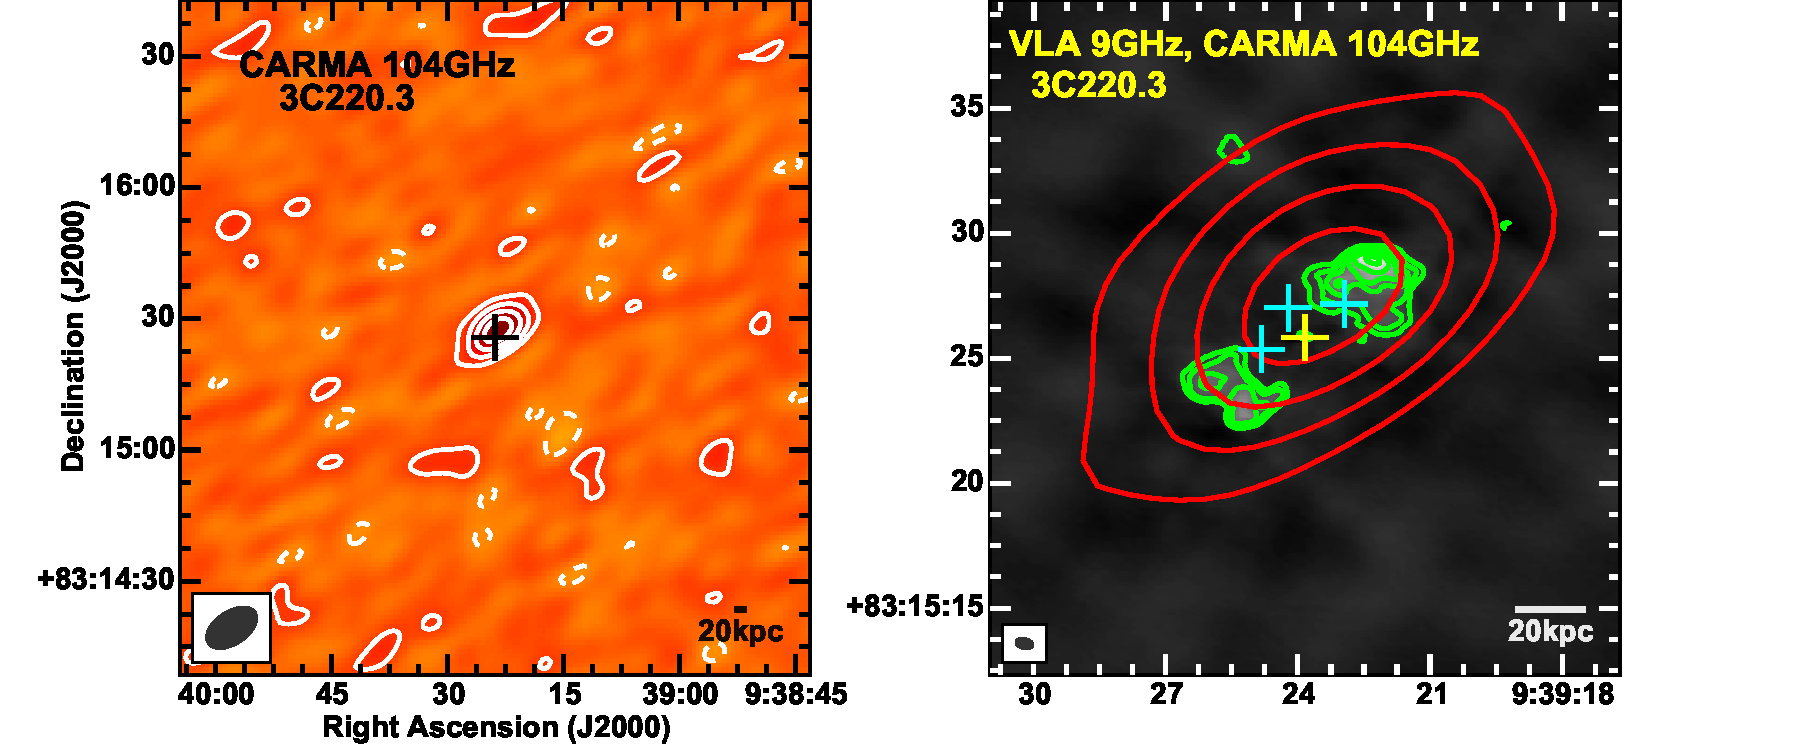
\includegraphics[width=0.80\textwidth]{Figure/ContPanel.pdf}
\caption{Left: Contour map of the 104 GHz continuum emission in 3C220.3. The beam size is 11\farcs9\,$\times$\,6\farcs5, at P.A.\,=\,
$-$56$\degr$, as indicated in the bottom left corner. Right: Contours of the CARMA 104 GHz continuum emission (red) from the 
foreground radio galaxy 3C220.3 overlaid on the 9 GHz emission (green contours and grayscale; H14). The synthesized beam size of the VLA observations is 0$\farcs$6\,$\times$\,0$\farcs$2, at P.A. 
76$\degr$. The central cross on each image indicates the position of the radio core of 3C220.3. The contour levels of the 104 GHz continuum emission start at $\pm$3$\sigma$, incrementing at steps 
of $\pm$1$\sigma$ of 0.5 mJy beam\pmOne; the contour levels of the 9 GHz continuum 
emission start at $\pm$4$\sigma$ where $\sigma$\,=\,0.064 mJy beam\pmOne\ and increment at steps of $\pm$2$^n\sigma$, 
where $n$ is a positive integer.
\label{fig:cont}}
\end{figure*}
%\subsection{New Results: \CO Line Emission}
\subsection{New Results: SMM\,J0939\\ \CO Line Emission}
We detect \CO line emission at $\sim$10(?yes?no?)$\sigma$ significance toward the background SMG SMM\,J0939 at $z$\,=\,2.221.
The spatial extent of this SMG is $\sim$5$\arcsec$, as shown in the Submillimeter Array (SMA) 1\,mm dust continuum in Figure \ref{fig:mom0}; as such, the detected \CO line emission is spatially unresolved. 
The line profile in Figure \ref{fig:mom0} is therefore extracted at the peak position of the unresolved CO emission. Fitting a four-parameter single Gaussian to the spectrum yields a peak flux density of 21.83\,$\pm$\,2.68\,\,mJy, superimposed on a continuum level of 4.19\,$\pm$\,0.49\,\,mJy, and full width at half-maximum (FWHM) of 557\,$\pm$\,36\,\,km\,\,s\pmOne. 
We construct a velocity-integrated (0th moment) map of the \CO line 
emission from the data after subtracting continuum emission in the visibility plane. This results in a velocity-integrated \CO line flux of $S_{\rm CO}$\,=\,10.7\,$\pm$\,1.3 Jy km\,\,s\pmOne\ over the FWZI velocity range of $\Delta v\sim$\,914 km\,\,s\pmOne, the uncertainty does not include $\sim$\,15\% calibration uncertainty. We ignore primary beam correction given that the source is close to the phase center and is unresolved (\ie much smaller than the primary beam size). Our \CO line measurement confirms the redshift of SMM\,J0939, yielding $z$\,=\,2.22122\,$\pm$\,0.00007.

\begin{figure*}[tbph] 
\centering
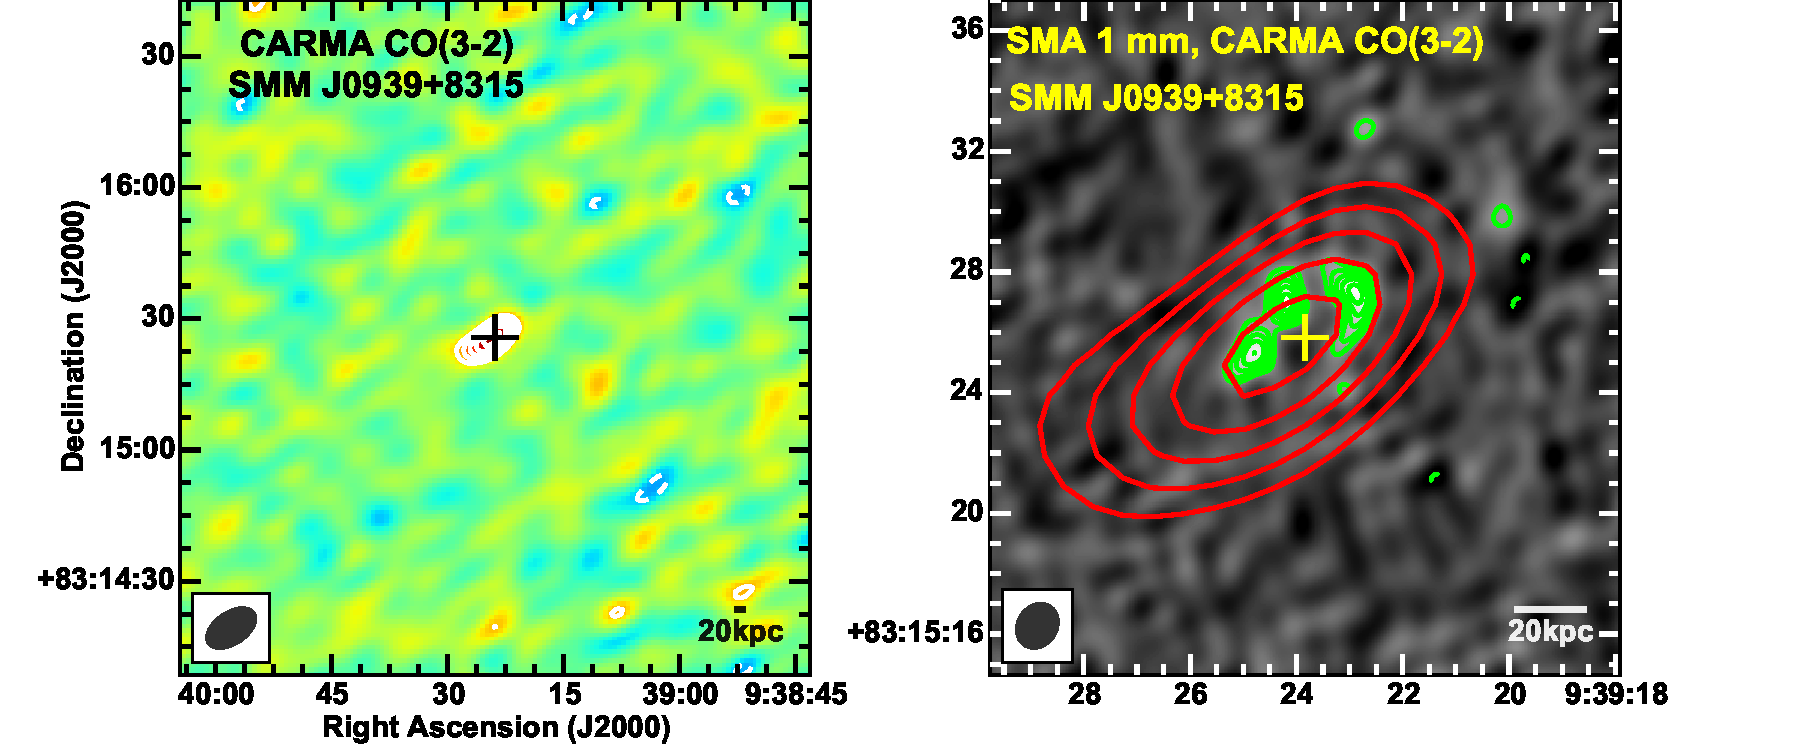
\includegraphics[width=0.8\textwidth]{Figure/LinePanel.pdf}
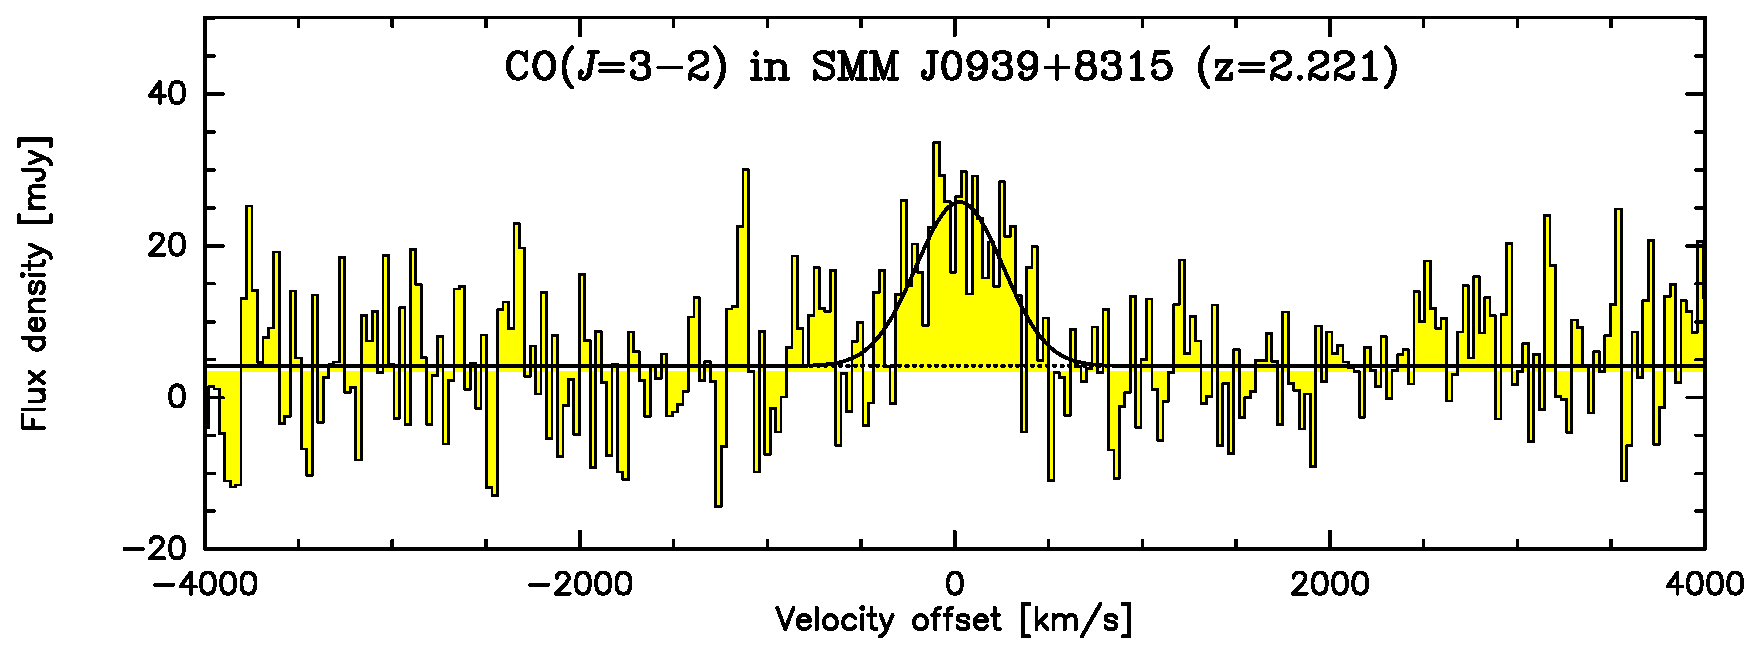
\includegraphics[width=0.65\textwidth]{Figure/smmj0939-co32_spec.eps}
\caption{Top Left: Continuum-subtracted moment-0 map of \CO line emission toward 
the background SMG with $\sigma$\,=\,1.00\,Jy\,\,km\,\,s\pmOne\ beam\pmOne\ over a velocity range of $\Delta v\sim$553\,km\,\,s\pmOne. The angular resolution is 11$\farcs$3\,$\times$\,6\farcs1, at P.A.\,=\,$-$56\degr, as indicated in the bottom left corner. 
Top Right: Contours of the \CO line emission (red) overlaid on the SMA 1\,mm dust continuum (green contours and grayscale; H14) with $\sigma_{\rm 1\,mm}$\,=\,0.84 mJy beam\pmOne. The beam size of the SMA data is 1\farcs4$ \times $1\farcs2, P.A. $-$34\degr, as shown 
in the bottom left corner. 
The central cross on each image corresponds to the same coordinates as in Figure \ref{fig:cont}. The contour levels start at $\pm$3$\sigma$, incrementing at
steps of $\pm$1$\sigma$. 
Bottom: 
Spectrum extracted at the peak position of CO line emission, with a spectral resolution of $\Delta v$ $\sim$29 km\,\,s\pmOne\, and an rms of $\sigma_{\rm ch}$\,=\,8.75 mJy beam\pmOne\ per channel.
Solid black line shows the Gaussian fit to the \CO line profile. Yellow histogram shows the 
flux density as a function of velocity offset, where the velocity scale is relative to $z$\,=\,2.221. 
%where 0 km\,\,s\pmOne\ corresponds to $z$\,=\,2.221. 
\label{fig:mom0}}
\end{figure*}


\section{Analysis}
\subsection{Lens Modelling} \label{sec:Lens} 
To study the intrinsic properties of the background galaxy, we determine the magnification factor by performing
lens modeling on the SMA 1\,mm archival data of this system. Lens modeling is carried out in the visibility
({\it uv-}) plane using the updated version\footnote{commit: 7aee6276} of the publicly available software {\sc uvmcmcfit}\footnote{https://github.com/sbussmann/uvmcmcfit}
\citep{Bussmann15a}. The code uses an affine-invariant Markov chain Monte Carlo (MCMC) approach to sample the posterior
probability density function (PDF) of the model parameters. In the code, the surface mass densities of both
lenses are represented by singular isothermal ellipsoid (SIE) profiles, and the source is assumed to have an
elliptical Gaussian profile. The code does not include an external shear parameter.

We fix the phase center to coordinates ($\alpha$,\,$\delta$)\,\,(J2000)\,=\,(9:39:23.54,\,\,83:15:26.10), the
angular offsets of the lenses and source are referenced to this phase center. The primary lens (3C220.3) is
described by five free parameters: the angular offset relative to
the chosen phase center in the image ($\Delta \alpha_{\rm
lens0}$ and $\Delta \delta_{\rm lens0}$), the angular Einstein radius ($\theta_{\rm E0}$), the
axial ratio ($q_{\rm lens0}$), and the position angle ($\phi_{\rm lens0}$). The secondary lens (companion B) is
described by three free parameters: $\theta_{\rm E1}$, $q_{\rm lens1}$, and $\phi_{\rm lens1}$. The angular offset
of the secondary
lens is sampled with respect to ($\Delta \alpha_{\rm lens0}$ and $\Delta \delta_{\rm lens0}$) of
the primary lens.
The source (SMM\,J0939) is parameterized by
six free parameters: the position of the source relative to the
primary lens ($\Delta \alpha_{\rm s}$ and $\Delta
\delta_{\rm s}$), the total intrinsic flux density ($S_\nu$), the
effective radius ($r_{\rm s}\,=\,\sqrt{a_{\rm s} b_{\rm s}}$), the axial
ratio ($q_{\rm s}$\,=\, $b_{\rm s}/a_{\rm s}$), and the position angle
($\phi_{\rm s}$).
The total number of free parameters is $N_{\rm free}$\,=\,14. The best-fit model is obtained by maximizing the
Gaussian likelihood function $ \mathcal{L} $ according to:
\begin{equation}
    \mathcal{L}\,=\,\sum_{u, v}\left( \frac{|V_{\rm data} - V_{\rm
    model}|^2}{\sigma^2} + {\rm log}(2 \pi \sigma^2) \right)
\end{equation}
\noindent where $\sigma$ is determined from the scatter in the visibilities within a
single spectral window (``natural" weighting).

We initialize the positions and Einstein radii of both lenses, and the position of the source using the
best-fit values of the lens model H14 performed on Keck K-band (near-infrared) data. For each of
these parameters, we impose a uniform prior in the range $\in\pm$3$\sigma$, where $\sigma$ is the uncertainty
reported in their paper. The axial ratios of the lenses are restricted to $q_{\rm lens} > 0.3$. We initialize 512
walkers and 6000 steps to identify the best-fit model parameters.
\begin{figure}[!tbpH]
\centering
\includegraphics[width=0.232\textwidth]{Figure/LensedSBmap_model_goodfit1970}
\includegraphics[width=0.232\textwidth]{Figure/LensedSBmap_residual_goodfit1970}
\caption{Double-lens modeling of SMM\,J0939 using {\sc uvmcmcfit} on the SMA 1\,mm continuum data.
The contours start at $\pm$2$\sigma$, incrementing at
steps of $\pm$2$\sqrt{\rm 2}\sigma$. Solid contours show the positive residuals and dashed contours
show the negative residuals. 
Left: SMA 1\,mm continuum (red contours) overlaid on the best-fit model (grayscale image) assuming an elliptical Gaussian profile for the background SMG. The lenses are represented as black dots, the half-light area of the background source is represented as magenta ellipse, and the critical curves are represented as orange curves. 
Right: Residual contours and image obtained by taking the Fourier transform of the difference between the SMA data and the best-fit model in the visibility plane. \label{fig:lens}}
\end{figure}

The resulting best-fit model as shown in Figure\,\,\ref{fig:lens} shows no significant bowls in the residual
image, and the knots (lensed emission) in the observed SMA data are well-reassembled with the best-fit model.
Our best-fit model yields a magnification
factor of $\mu_{\rm L}$\,=\,10.13\,$\pm$\,1.38, this is consistent the value reported by H14 within the errors. All best-fit
parameters are listed in Table \ref{tab:lensParam}. The Einstein radii associated with the best-fit model for the two lenses are $\theta_{E}$\,=\,1.22\,$\pm$\,0.01 (8.75 kpc at $z$\,=\,0.685) and $\theta_{E}$\,=\,0.75\,$\pm$\,0.02 (5.34 kpc at $z$\,=\,0.685),
the corresponding masses within the Einstein radii are $M(\theta$\,\,$<$\,\,$\theta_{\rm E})$\,=\,(4.86\,$\pm$\,0.08)\,$\times$\,10$^{11}$\,\,\Msun\ and $M(\theta$\,\,$<$\,\,$\theta_{\rm E})$\,=\,(1.82\,$\pm$\,0.07)\,$\times$\,10$^{11}$\,\,\Msun, respectively. 
\begin{deluxetable}{l l r}[tbpH]
\tabletypesize{\scriptsize}
\tablecolumns{3}
\tablewidth{0pc}
\tablecaption{Lens modeling results}
\tablehead{
\multicolumn{2}{c}{Parameters} &
\colhead{Best-Fit Values}
\\ \cline{1-3} \vspace{-0.05in} \\
% \tableline
\multicolumn{3}{c}{Lens 0}
}
\startdata
%\cutinhead{Lens 0}
$\Delta \alpha_{\rm lens0}$      & (\arcsec)   & 0.403 $\pm$ 0.026     \\
$\Delta \delta_{\rm lens0}$      & (\arcsec)   & -0.181 $\pm$ 0.027    \\
$q_{\rm lens0}$ \tablenotemark{a} &             & 0.446 $\pm$ 0.063     \\
$\phi_{\rm lens0}$                & (deg)       & 31.56 $\pm$ 4.15\phn  \\
$\theta_{\rm E0}$                & (\arcsec)   & 1.218 $\pm$ 0.010     \\
\cutinhead{Lens 1}
$\Delta \alpha_{\rm lens1}$       & (\arcsec)   & -0.804 $\pm$ 0.034    \\
$\Delta \delta_{\rm lens1}$       & (\arcsec)   & -1.243 $\pm$ 0.017    \\
$q_{\rm lens1}$ \tablenotemark{a} &             & 0.608 $\pm$ 0.138     \\
$\phi_{\rm lens1}$                & (deg)       & 14.2 $\pm$ 15.7\phn      \\
$\theta_{\rm E1}$                & (\arcsec)   & 0.745 $\pm$ 0.015     \\
\cutinhead{Source}
$\Delta \alpha_{\rm s}$           & (\arcsec)   &  -0.163 $\pm$  0.035   \\
$\Delta \delta_{\rm s}$           & (\arcsec)   & -0.193 $\pm$  0.048   \\
$q_{\rm s}$ \tablenotemark{a}     &             & 0.424 $\pm$ 0.237     \\
$\phi_{\rm s}$                    & (deg)       & 174.34 $\pm$ 8.89\phn \\
$r$\tablenotemark{b}              & ($\arcsec$) & 0.106 $\pm$   0.033   \\
$\mu$                             &             & 10.13 $\pm$ 1.38\phn
\enddata
% 0.377 & -0.209 & 0.446 & 33.22 & 1.223 & -0.788 & -1.26 & 0.5289 & 9.55 & 0.733 & 9.74
\label{tab:lensParam}
\tablenotetext{a}{Axial ratio}
\tablenotetext{b}{Effective Radius}
% \tablenotetext{c}{}
\tablecomments{The angular offsets listed above are with respect to $\alpha$ = 9:39:23.54, $\delta$ = 83:15:26.10 (J2000). }
\end{deluxetable}

















\subsection{SED Fitting} \label{sec:SED}
\subsubsection{3C220.3}\label{sec:SEDFg}
Synchrotron continuum emission from extended components of a radio galaxy decreases with increasing radio frequencies, 
and the spectrum is commonly characterized by a power law distribution $S \propto \nu^{-\alpha}$, where the 
spectral index $\alpha$ is $\gtrsim$ 0.5. While the contribution from extended components decreases, studies using 
samples of radio galaxies have suggested that the flat/inverted-spectrum of the compact radio core component rises 
and dominates the flux density at higher frequencies \citep{Kellermann81a,Begelman84a}. This has been observed in a FR-II galaxy at a similar redshift\,--\,3C220.1 at the redshift of $z$\,=\,0.610, where observations were carried out at observed-frame $\sim$\,90 GHz \citep{Hardcastle08a}. It is noteworthy that prior to our observations, 3C220.1 was the only FR-II galaxy with high frequency radio observations at $z$\,$>$\,0.6. Previous studies of the core component of 3C220.3 have established upper 
limit of $<$ 0.17 mJy at 4.6 GHz \citep{Mullin06a} and an unambiguous detection of 0.8 mJy at 9 GHz (H14), suggesting a substantially inverted spectrum of the core (Figure \ref{fig:SED}).
Consequently, we may naively expect the integrated flux density in our continuum detection of $S_{\rm 104GHz}$\,=\,9.46\,$\pm$\,0.64\,\,mJy to be dominated by the unresolved core component of the foreground FR-II galaxy, which is at $z$\,=\,0.685. 
However, the deconvolved spatial size of the source matching that in the resolved image (see Figure 1) is 
suggestive of a marginally resolved detection of the extended components with non-negligible emission. 
This is plausible given that the orientation of the synthesized beam in our observations is in alignment with the 
axis along the 
lobes of the radio galaxy, as shown in Figure \ref{fig:cont}. We investigate this disparity by fitting models to 
existing SED data of the total integrated flux as listed in Table \ref{tab:SEDdataRadio}, and extrapolating the fit to 
estimate the flux density of the lobes at the frequency of our continuum measurement. 
\begin{deluxetable}{rlrcc}[tbpH]
\tabletypesize{\scriptsize}
\tablecolumns{5}
\tablecaption{Continuum data of 3C220.3}
\tablehead{
\multicolumn{2}{c}{Frequency} &
\multicolumn{2}{c}{Flux Density} &
\colhead{Reference} \vspace{0.05in}
\\  \cline{1-5} \vspace{-0.05in} \\
\multicolumn{5}{c}{Integrated (Core \& Lobes)}
}
\startdata
    104.2 & GHz & 7.39 $\pm$ 1.42\tna        & mJy & LR15 \\
%    104.2 & GHz & 4.91 $\pm$ 0.54\tna        & mJy & This work \\
    10.7  & GHz & 270 $\pm$ 30            & mJy & KP73       \\
    10.7  & GHz & 253 $\pm$ 28            & mJy & L80       \\
    5.0   & GHz & 640 $\pm$ 100           & mJy & K69       \\
    5.0   & GHz & 636 $\pm$ 50            & mJy & L80       \\
    2.7   & GHz & 1.33 $\pm$ 0.07         & Jy  & K69       \\
    2.7   & GHz & 1.34 $\pm$ 0.10         & Jy  & L80       \\
    1.4   & GHz & 2.95 $\pm$ 0.09         & Jy  & C98       \\
    1.4   & GHz & 2.99 $\pm$ 0.06         & Jy  & P66       \\
    1.4   & GHz & 2.80 $\pm$ 0.14         & Jy  & K69       \\
    1.4   & GHz & 2.89 $\pm$ 0.09         & Jy  & L80       \\
    0.75  & GHz & 5.94 $\pm$ 0.28         & Jy  & L80       \\
    0.75  & GHz & 5.94 $\pm$ 0.21         & Jy  & P66       \\
    0.75  & GHz & 5.60 $\pm$ 0.84         & Jy  & K69       \\
    352   & MHz & 11.3 $\pm$ 0.453        & Jy  & WENSS     \\
    352   & MHz & 11.6 $\pm$ 0.464        & Jy  & WENSS     \\
    178   & MHz & 15.7 $\pm$ 2.35         & Jy  & K69       \\
    178   & MHz & 17.1 $\pm$ 1.71         & Jy  & L80       \\
    152   & MHz & 22.6 $\pm$ 0.08         & Jy  & B85       \\
    152   & MHz & 22.5 $\pm$ 0.04         & Jy  & B85       \\
    86    & MHz & 51.6 $\pm$ 9.90         & Jy  & L80       \\
    73.8  & MHz & 37.5 $\pm$ 3.82         & Jy  & C07       \\
    38    & MHz & 49.6 $\pm$ 4.96         & Jy  & L80       \\
    38    & MHz & 40.2 $\pm$ 6.30         & Jy  & K69       \\
    37.8  & MHz & 60.7 $\pm$ 6.07         & Jy  & H95       \\
    17.8  & MHz & 64.9 $\pm$ 6.49         & Jy  & H95			\\
\cutinhead{Core Only}
    104.2 & GHz & $<$ 2.29 		      & mJy & LR15 \\
    9.0   & GHz & 0.80  $\pm$ 0.06    & mJy & H14       \\
    4.86  & GHz & $<$ 0.17            & mJy & M06       \\
\enddata
\label{tab:SEDdataRadio}
\tablenotetext{a}{Integrated flux density. Peak flux density of the continuum emission is 4.93 $\pm$ 0.31 mJy beam\pmOne}
%\tablenotetext{b}{Core only}
\tablenotetext{$\dagger$}{www.astron.nl/wow/testcode.php?survey=1}
%\tablecomments{References.~}
\tablerefs{
B85 = \citet{r2728};
C98 = \citet{r16};
C07 = \citet{r30};
H95 = \citet{r33-34};
H14 = \citet{Haas14};
K69 = \citet{r11-14-18-22-25-32};
KP73 = \citet{r9};
L80 = \citet{r10-13-15-19-20-26-29-31};
LR15 = this work;
M06 = \citet{Mullin06a};
P66 = \citet{r17-21};
WENSS = \citet{r23-24}$^\dagger$
}
\end{deluxetable}
















Following Equation (1) in \citet{Cleary07a}, the fit to the lobe emission can be expressed as a parabolic function:
\begin{equation}
\log F_{\nu}^{\mathrm lobe} (\nu) \propto - \beta\ (\log\ \nu - \log \nu_{t})^2  + \log (\exp({\frac{\nu}{\nu_c^{\mathrm lobe}}}))
\end{equation}
where $F_{\nu}^{\mathrm lobe}$ is the flux density of the lobes, $\beta$ is a parameter representing the bending 
of the parabola, $\nu_t$ is the frequency at which the optical depth of the synchrotron emitting plasma reaches 
unity, and $\nu_c^{\rm lobe}$ is the frequency corresponding to the cutoff energy of the lobe plasma energy 
distribution. 
The extrapolated flux density at 104\,\,GHz is consistent with the peak flux density of our continuum 
measurement (Figure \ref{fig:SED}). The 9$\sigma$ detection of the continuum thereby suggests
a dominant contribution from the lobes, and the peak flux density does not appear to be emission toward 
the core. Moreover, the peak position of the 104\,\,GHz continuum is
centered toward the northern lobe (Figure \ref{fig:cont}), which further supports our argument. We did not 
extrapolate the core measurements to the frequency of our continuum, as previous measurements of the core are 
taken 
across different epochs. 
We place an upper limit of $S_\nu$\,$<$\,4.28 mJy on the core component using the difference in flux density.
\par
Studies by \citet{Meisenheimer89a} and \citet{Hardcastle08a} have suggested spectra of hotspots are flat up to optical frequencies, where some exhibit spectral steepening in cm and mm wavelengths (\eg 3C123). At the resolution of our observations, it is unclear whether the flux density is dominated by the emission from the compact hotspot or the emission from the surrounding diffuse lobe components.

\begin{figure}[!tbph]
\centering
\includegraphics[width=0.5\textwidth]{Figure/3C220_3_FullSED2_longticks.pdf}
\caption{The SED of 3C220.3 (solid purple line) and SMM\,J0939 (dashed purple line and solid cyan line) including the new measurements presented in this paper. 
Black dots represent existing data of 3C220.3 (see Table \ref{tab:SEDdataRadio}). Red dots at 104 GHz correspond to 
our continuum measurements (integrated, peak, and difference). The purple line corresponds to the parabolic function we 
fit to the data associated with the radio galaxy, following \citet{Cleary07a}. The dashed purple line and 
the solid cyan line correspond to the best-fit SED models of the background SMG. The photometric data of the SMG are reported by H14. \label{fig:SED}}
\end{figure}

\subsubsection{SMM\,J0939+8315} \label{sec:SEDBg}
To constrain the dust and gas properties in the ISM of SMM\,J0939, we perform SED fitting to the
photometric data obtained with {\it Herschel}/PACS and SPIRE, at wavelengths
between observed-frame 70 \micron\,$-$\,500 \micron, and the interferometric data obtained with the SMA at 1\,mm (H14). We use the publicly
available software {\sc mbb\_emcee}\footnote{https://github.com/aconley/mbb\_emcee} to perform the SED fitting; the code uses an affine-invariant Markov chain Monte
Carlo (MCMC) approach, further details of the code are given by \citet{Riechers13a} and \citet{Dowell14a}. The
functional form of the fit comprises a single-temperature, modified blackbody function joined to a $S_{\lambda} \propto \lambda^\alpha
$ power law on the blue
side of the SED.
We fit both optically thick and optically thin models. In the optically thick case, the wavelength $
\lambda_0$\,=\,${c}/{\nu_0}$ is an additional parameter representing the rest-frame wavelength at which the optical
depth $\tau_{\nu} =$ ($\nu$/$\nu_0$)$^\beta$ reaches unity. Thus, the functional form of the modified blackbody
in the optically thick regime is as follows:
\begin{equation}
\rm S_{\lambda} \propto \frac{(1-exp^{-(\frac{\lambda_0 (1+z)}{\lambda})^{\beta}})(\frac{c}{\lambda})^3}
{exp^{\frac{hc}{\lambda\rm{kT/(1+z)} } }-1}
\end{equation}
and in the optically thin regime, the functional form reduces to:
\begin{equation}
\rm S_{\lambda} \propto \frac{(\frac{c}{\lambda})^{\beta+3}}{exp^{\frac{hc}{\lambda\rm{kT/(1+z)}}}-1}
\end{equation}
where $T$ is the rest-frame characteristic cold dust temperature, $\beta$ is the dust emissivity (or spectral index of the dust extinction
curve), and $\alpha$ is the power law spectral index. The overall fit is normalized using the observed-frame 500
$\micron$ flux density, hence this becomes an additional parameter in the fit. For both models, we impose an upper limit on the observed-frame dust temperature ($T/(1+z)$) to 60 K, and for the optically thick model, we impose an upper limit on $\lambda_0$ to 2000\,\,\micron. Additionally, we fix the upper limits on 
$\beta$ to be 3.0 and 2.2 for the optically thin model and optically thick model, respectively.

\begin{deluxetable}{ccc}[tbpH]
\tabletypesize{\scriptsize}
\tablecolumns{3}
\tablecaption{SED fitting results}
\tablehead{
\colhead{Parameters}                  &
\colhead{Optically Thick}       &
\colhead{Optically Thin}
}
\startdata
$\chi^2$ & 2.25 & 5.31 \\
D.O.F & 2 & 3 \\
$T_{\rm d}$ (K) & 60.91$^{+1.08}_{-1.31}$ & 51.95$^{+1.26}_{-1.21}$ \\
$\beta$ & 1.35$^{+0.57}_{-0.53}$ & 0.7$^{+0.24}_{-0.26}$ \\
$\alpha$ & 3.05$^{+0.31}_{-0.40}$ & 2.76$^{+0.23}_{-0.23}$ \\
%$\lambda_0$(1+$z$) ($\micron$) \tablenotemark{c} & 722.81$^{+276.88}_{-398.67}$ & --- \\
$\lambda_0$ ($\micron$) \tablenotemark{e} & 224.41$^{+85.96}_{-123.77}$ & --- \\
$\lambda_{\rm peak}$ \tablenotemark{c}\micron & 254.7$^{+6.2}_{-6.1}$ & 301.4$^{+29.0}_{-30.1}$ \\
$f_{\rm norm, 500 \micron}$ mJy  \tablenotemark{c} & 255.79$^{+16.67}_{-16.31}$ & 244.25$^{15.28}_{15.30}$ \\
$L_{\rm (8-1000)\micron}$ [10$^{12}$ L$_\sun$] \tablenotemark{d} & 88.52$^{+2.62}_{-2.63}$ & 89.15 \\
$M_{\rm d}$ [10$^8$ M$_\odot$] \tablenotemark{b} & 50.47$^{+20.42}_{-20.15}$ & 25.74$^{+3.88}_{-5.49}$
\enddata

% Optically thick & 18.91 & 1.35 & 722.81 & 3.05 & 254.7 & 88.52 & 50.47 \\
% Optically thin &  16.13 & 0.7 & N/A   & 2.76 & 301.4 & 89.15 & 25.74

\label{tab:mbb}
\tablenotetext{a}{The observed-frame wavelength where the dust becomes optically thick}
\tablenotetext{b}{Assuming standard absorption mass coefficient $\kappa$=2.64 m$^2$ kg$^{-1}$ at $\lambda$=125.0 $\micron$ (Dunne et al. 2003), without lensing correction}
\tablenotetext{c}{observed-frame}
\tablenotetext{d}{rest-frame 8-1000 $\micron$ without lensing correction}
\tablenotetext{e}{The rest-frame wavelength where the dust becomes optically thick, upper limit is 2000 $\micron$}
\tablecomments{Errors are $\pm$1$\sigma$}
\end{deluxetable}

% thick_500_500.log
% T/(1+z): 18.91 +1.09 -1.31 (low lim: 1.00 upper lim: 60.00) [K]
% beta: 1.35 +0.57 -0.53 (low lim: 0.10 upper lim: 2.20)
% fnorm: 255.79 +16.67 -16.31 (low lim: 0.03) [mJy]
% lambda0 (1+z): 722.81 +276.88 -398.67 (low lim: 1.00 upper lim: 3049.15) [um]
% alpha: 3.05 +0.31 -0.40 (low lim: 0.10 upper lim: 20.00)
% Lambda peak: 254.7 +6.2 -6.1 [um]
% L_IR(8.0 to 1000.0um): 88.52 +2.62 -2.63 [10^12 L_sun]
% M_d(kappa=2.64, lam=125.0um): 50.47 +20.42 -20.15 [10^8 M_sun]
% Number of data points: 7
% ChiSquare of best fit point: 2.25

% note using beta upper limit 3.0, getting very different beta, and dust mass
% Fit results:
% T/(1+z): 19.75 +0.56 -0.53 (low lim: 1.00 upper lim: 60.00) [K]
% beta: 1.91 +0.76 -0.76 (low lim: 0.10 upper lim: 3.00)
% fnorm: 267.13 +16.03 -15.98 (low lim: 0.03) [mJy]
% lambda0 (1+z): 1012.99 +142.79 -275.29 (low lim: 1.00 upper lim: 3049.15) [um]
% alpha: 3.64 +0.08 -0.86 (low lim: 0.10 upper lim: 20.00)
% Lambda peak: 255.6 +6.3 -6.2 [um]
% L_IR(8.0 to 1000.0um): 88.02 +2.85 -2.85 [10^12 L_sun]
% M_d(kappa=2.64, lam=125.0um): 108.23 +32.00 -63.67 [10^8 M_sun]
% Number of data points: 7
% ChiSquare of best fit point: 2.25
% Saving results to thick_testbeta.h5

% thin_testSMA
% T/(1+z): 16.13 +1.26 -1.21 (low lim: 1.00 upper lim: 60.00) [K]
% beta: 0.70 +0.24 -0.26 (low lim: 0.10 upper lim: 3.00)
% fnorm: 244.25 +15.28 -15.30 (low lim: 0.03) [mJy]
% alpha: 2.76 +0.23 -0.23 (low lim: 0.10 upper lim: 20.00)
% Lambda peak: 301.4 +29.0 -30.1 [um]
% L_IR(8.0 to 1000.0um): 89.15 +2.48 -2.51 [10^12 L_sun]
% M_d(kappa=2.64, lam=125.0um): 25.74 +3.88 -5.49 [10^8 M_sun]
% Number of data points: 7
% ChiSquare of best fit point: 5.31

The best-fit values in both regimes are listed in Table \ref{tab:mbb}, and the correlation plots are available in the Appendix. The best-fit solution of an optically thin
model corresponds to $\chi^2$\,=\,5.31 with 3 degrees of freedom, whereas that of an optically thick model
corresponds to $\chi^2$\,=\,2.25 with 2 degrees of freedom, suggesting a better fit than in the optically thin
case. In the subsequent analysis, we employ the inferred values from the optically thick model.
The best-fit solution yields a rest-frame FIR luminosity of $L_{\rm FIR (42.5-122.5\micron)}$\,=\,53.3$^{+1.1}_{-1.1}$\,$\times$\,10$^{12}$\,\Lsun, and a total infrared (IR) luminosity of $L_{\rm IR (8-1000 \micron)}$\,=\,88.5$^{+2.6}_{-2.6}$\,$\times$\,10$
^{12}$\,\Lsun. Assuming a dust absorption coefficient of $\kappa_{\nu}$\,=\,2.64 m$^2$ kg\pmOne\ at 125.0 $
\micron$ \citep{Dunne03a}, we derive the dust mass using the following expression:
\begin{equation}
M_{\rm dust}\,=\,S_{\nu} D_{L}^2 [(1 + z) \kappa_{\nu} B_{\nu}]^{-1} \tau_{\nu} [1-
\exp(-\tau_{\nu})]^{-1}
\end{equation}
where $S_{\nu}$ is the flux density in ergs/s/cm$^{2}$/Hz , $D_{\rm L}$ is the luminosity distance in cm, $\kappa_{\nu}$ is the dust
absorption coefficient in cm$^2$ g\pmOne, $\tau_{\nu}$ is the optical depth, and $B_{\nu}$ is the Planck function,
all quantities are expressed in the observed-frame. We find a dust mass of $M_{\rm dust}$\,=\,50.5$^{20.4}_{-20.2}\times$10$^8$\,\,\Msun, the uncertainties do not include those of $\kappa_{\nu}$. These values are based on SED fitting to the photometric data, \ie prior
to lensing correction. 

With the limited amount of data in the FIR waveband, the dust mass is weakly constrained. 
We perform an additional fit using an optically thick model where we loosen the upper limit of $\beta$ from 2.2 to 3.0, while the difference between all best-fit parameters in this scenario and those using an upper limit of 2.2 (see Table \ref{tab:mbb}) is within 3\%, we find that the dust mass is boosted by a factor of $\sim$2. 

\subsection{Molecular Gas Mass}
While the ground state CO transition line, CO($J$\,=\,1 \rarr\ 0) traces the cold molecular gas in the ISM
\citep*[\eg][]{Wilson70a,Downes98a}, CO($J$ $>$ 1) transition lines are frequently observed at high redshifts as the
 ground state CO transition line is redshifted to lower frequencies that can only be observed with a few telescopes 
 \citep{Carilli13a}, 
 hence assumptions on the CO excitation conditions are required to derive the molecular gas mass using the H$_{\rm 2}$-to-CO 
 relation. 
Prior to the observations of the ground state CO line in SMGs, it has been assumed that the molecular gas in the
  ISM traced by CO lines is thermalized due to their high star formation rates \citep[\eg][]{Greve05a, Coppin08a}.
   Yet, recent observations of this line have demonstrated that SMGs can indeed be subthermally excited
   \citep{Harris10a,Riechers11c,Riechers11d,Ivison11a}; based on observations toward SMGs of both the \CO and the CO($J$\,=\,1 \rarr\ 0) lines, the 
   brightness temperature ratio has been inferred as $R_{\rm 31}<$ 0.8 \citep
   {Harris10a,Carilli10a,Swinbank2010a,Riechers11d,Ivison11a,Ivison10d}. In contrast, observations of high-redshift quasar hosts suggest that the ratio 
   is $R_{\rm 31}\sim$ 1 \citep{Riechers06a, Riechers11a, Scott11a}. 
Here, we derive the molecular gas mass 
assuming thermalized excitation of CO, 
\eg we adopt $R_{\rm 31}$\,=\,1 as SMM\,J0939 is 
postulated to be hosting a type-2 quasar; this is based on the reported brightness temperature ratio of $R_{\rm 31}$\,=\,1.00\,$\pm$\,0.10 for the type-2 quasar host IRAS F10214+4724 \citep{Riechers11a}.
\par
We calculate the CO($J$\,=\,1 \rarr\ 0) line luminosity using standard relation 
\citep[\eg][]{Solomon05a,Carilli13a}:
\begin{equation}
L^{\prime}_{\rm CO}\,=\,\frac{3.25\times10^7}{\nu_{\rm CO (3-2)}^2}\times \frac{D_L^2}{\mu} \times
\frac{I_{\rm CO(3-2)}} {R_{\rm 31} (1 + z)}
\end{equation}
where $\nu_{\rm CO (3-2)}$ is the rest-frame frequency of the \CO transition line in GHz, $D_L$ is the luminosity distance in Mpc, and $I_{\rm CO(3-2)}$ is the \CO line flux in Jy\,\,km\,\,s\pmOne. After correcting for lensing magnification, this corresponds to $L^{\prime}_{\rm CO (1-0)}$\,=\,(2.91\,$\pm$\,0.60)\,\,$\times$\,\,10$^{10}$\,(10.1/$\mu_{\rm L}$)\,\,\LpU; the inferred total molecular gas mass is therefore $M_{\rm gas}$\,=\,(2.33\,$\pm$\,0.48)\,\,$\times$\,\,10$^{10}$\,\Msun. We assumed a conversion factor of $\alpha_{\rm CO}$\,=\,0.8\,\,\Msun\,(\LpU)\pmOne\ based on empirical relations from local ULIRGs, which is typically
adopted for SMGs \citep[\eg][]{Tacconi06a,Tacconi08a,Bothwell13a}. 
This results in a gas-to-dust
ratio of $f_{\rm gas-dust}$\,=\,$M_{\rm gas}/M_{\rm dust}$\,=\,47\,$\pm$\,21, in good agreement with the 
values found in other SMGs \citep{Coppin08a,Micha10a,Riechers11c}.
% find an excellent agreement of blah with blah
\subsection{Star Formation Rate}
No strong evidence of a warm dust component is found in SMM\,J0939 based on the mid-IR continuum measurements (see Figure \ref{fig:SED}), hence we derive the star formation rate (SFR) assuming negligible contributions to the IR luminosity due to AGN heating. 
Using the \citet{Kennicutt98a} relation and assuming \citet{Chabrier03a}
stellar initial mass (IMF) function\footnote{SFR$_{\rm FIR}$\,=\,526\,$\pm$\,73 $M_
\odot$ yr\pmOne\ }, 
the SFR$_{\rm IR}$ is 874\,$\pm$\,122\,\,$M\sun$\,\,yr\pmOne.
Assuming constant SFR, the time for which the starburst in SMM\,J0939 can be maintained at its
current SFR can be approximated as the gas depletion timescale, $\tau_{\rm depl}$\,=\,$M_{\rm gas}$/SFR. 
This corresponds to $\tau_{\rm depl}$\,=\,25.6\,$\pm$\,0.4 Myr, which is in good agreement with those found in other SMGs \citep[\eg][]{Greve05a}. 

\subsection{Star Formation Efficiency}
The SFR per unit mass of molecular gas is commonly taken as a
measure of the star formation efficiency, SFE\,=\,SFR/$M_{\rm gas}$. We compute this ratio using lensing-corrected IR 
luminosity and CO luminosity, i.e., SFE\,=\,$L_{\rm IR}$/\Lp, this makes no assumptions on the CO luminosity to gas mass conversion factor ($\alpha_{\rm CO}$) as well as the 
choice of IMF, however, this assumes that differential lensing effect between the CO and infrared emission is negligible. 
The resulting ratio is SFE$_{\rm IR}$\,=\,300\,$\pm$\,9\,\,\Lsun\,(\LpU)$^{-1}$, this is comparable
to what is found in ``typical" SMGs \citep{Riechers11c,Greve05a,Tacconi06a}.

\subsection{Dynamical Mass} 
Based on our \CO line measurement, we can estimate the dynamical mass of SMM\,J0939 using an isotropic virial estimator \citep[\eg][]{Engel10a}:
\begin{equation}
M_{\rm dyn}\,=\,2.8\times 10^5\Delta v_{\rm line}^ 2 R_{\rm eff}
\end{equation}
where $\Delta v_{\rm line}$ is in km\,\,s\pmOne, $R_{\rm eff}$ is in kpc, and $M_{\rm dyn}$ is in \Msun.
We employ the FWHM linewidth of the \CO line profile for $\Delta v_{\rm line}$,
and the half-light radius from our lens model for $R_{\rm eff}$, this assumes that the dust emission traces the same emitting region as the CO. The inferred dynamical mass is $M_{\rm dyn}$\,=\,(7.4\,$\pm$\,2.4)\,$\times$\,10$^{10}$\,\Msun, and the gas-to-dynamical mass fraction is $f_{\rm gas-to-dyn}$\,=\,0.32\,$\pm$\,0.12, this is consistent with that of other SMGs \citep{Tacconi06a}.

\subsection{Star Formation and Gas Surface Densities}
To compute surface densities, we divide half the inferred SFR and gas mass by the area subtended by the half-light 
radius, resulting in $\Sigma_{\rm gas}$\,=\,4.67\,$\times$\,10$^9$\,\,\Msun\,\,kpc$^{-2}$ and $\Sigma_{\rm SF}$\,=\,175.20\,\,\Msun\,\,yr\pmOne\,\,kpc$^{-2}$, in good agreement with values typical for SMGs \citep{Tacconi08a}. 

The inferred surface densities of SMM\,J0939 follow a universal Schmidt-Kennicutt relation between the star formation rate
surface density and the molecular gas surface density reported by \citet{B07a}: $\Sigma_{\rm SF}$\,=\,9.3\,$\times$\,10$^{-5}$ ($M_{\rm gas}$/2$\pi R_{\rm 1/2}^2)^{1.71}$, which was derived using a sample consisting of local star-forming galaxies and high-redshift 
galaxies
out to $z\ \sim$ 2.5, and assuming Chabrier IMF. 

\section{Discussion And Conclusions} \label{sec:conclusions}
We present the detection of \CO line emission toward SMM\,J0939+8315, a strongly lensed SMG that is hosting a type-2 quasar, refining the redshift of this SMG to $z$\,=\,2.22122\,$\pm$\,0.00007. The peculiarity of this system allows us to put constraints on the SED of 3C220.3 using the underlying continuum detection at $\sim$104 GHz, making this the second high frequency radio continuum measurement of FR-II galaxy at $z$ $>$ 0.6. We argue that the detected peak continuum emission is dominated by the emission from the lobes and hotspots, we therefore place an upper limit of $S_\nu$ $<$ 4.28 mJy on the radio core. 

The detection of CO in SMM\,J0939 
implies a CO luminosity of \Lp\,=\,2.91\,$\pm$\,0.60\,$\times$\,10$^{10}$(10.1/$\mu_{\rm L}$)\,\,\LpU\, suggesting the presence of a large molecular gas reservoir; the inferred high SFR of $\sim$ 874 \Msun\ yr\pmOne 
 SMM\,J0939 is undergoing 
active star formation, which is typical for SMGs, 
which supports the picture that SMGs are a 
population of high-z galaxies that spawn most of the stellar mass in the early universe, thus play an important role 
in galaxy evolution and formation. 

The detection of thermal dust emission in SMM\,J0939 implies a FIR Luminsoity of 
Assuming the dominant heating mechanism is from young, massive stars, then the SFR implied from the LIR is blah
From the IR continuum data, we expected contribution to the bolometric IR luminosity due to heating of the dust-enshrouded AGN is minor, the physical properties are therefore derived using the lensing-corrected bolometric IR luminosity. The high dust temperature is unusual for SMGs, but not unseen. 

Lensing prbes the brightess apparent 
Regardless of lensing, the inferred intrinsic properties of SMM\,J0939 shows that this SMG is representation of the population.
\newcommand\tnh{\,\tablenotemark{h}}
\newcommand\tni{\,\tablenotemark{i}}
\newcommand\tnj{\,\tablenotemark{j}}
\newcommand\tnk{\,\tablenotemark{k}}
\begin{deluxetable*}{l l c c c c c}[tbpH]
\tabletypesize{\scriptsize}
\tablecolumns{7}
\tablecaption{Comparison of SMM J0939 with SMGs at $z\sim$2}
\tablehead{
\multicolumn{2}{c}{SMGs}       &
\colhead{SMM J0939}  &
\multicolumn{2}{c}{HLSW-01}    &  
\multicolumn{2}{c}{Cosmic Eyelash} 
                     \\
\colhead{Quantity} &
\colhead{Unit} &
\colhead{}                     &
\colhead{}                     &
\colhead{Ref.}                     &
\colhead{}                     &
\colhead{Ref.}
}
\startdata
$z$             &                   & 2.221            & 2.957            & R11              & 2.326          &  S10 \\
$\mu_{\rm L}$         &                   & 10.1 $\pm$ 1.4    & 10.9 $\pm$ 0.7 & G11              & 37.5$\pm$4.5    &  S11 \\
$S_{\rm 250}$ & mJy & 440 $\pm$15 (H14) & 420 $\pm$ 10  & R11              & 366 $\pm$ 55  & I10             \\
$I$\tnb       & Jy km s$^{-1}$   & 10.7 $\pm$ 2.1   & 9.7 $\pm$ 0.5  & R11              & 13.2 $\pm$ 0.1 &  D11 \\
$\Delta v_{\rm FWHM}$\tnb & km s$^{-1}$ & 542 $\pm$ 32 & 350 $\pm$ 25 & R11 & $\lesssim$ 800\tnd & D11 \\
\Lp & 10$^{10}$ \LpU & 2.91 $\pm$ 0.78\tnh & 4.17 $\pm$ 0.41 & R11 & 1.7 $\pm$ 0.2 & D11 \\
$M_{\rm gas}$ & 10$^{10}$ \Msun & 2.33 $\pm$ 0.62\tnh & 3.3 $\pm$ 0.3 & R11 & 1.6 $\pm$ 0.1 & I10 \\
$L_{\rm IR}$ &  10$^{12}$ \Lsun & 9.1 $\pm$ 1.2\tnh & 14.3 $\pm$ 0.9 & C11 & 2.3 $\pm$ 0.2 & I10 \\
$M_{\rm dust}$ & 10$^8$ \Msun & 5.2 $\pm$ 2.1\tnh  & 1 - 5.2
& R11 & $\sim$4.0 & I10 \\
SFR$_{\rm IR}$\tna & \Msun yr$^{-1}$ & 874 $\pm$ 122\tnh & 1430 $\pm$ 160\tnc & C11 & $\sim$235\tnc & I10 \\
$\tau_{\rm depl}$\tng & Myr & 25.6 $\pm$ 0.6 & 23 $\pm$ 3\tnc  & R11 & 68\tne & --- \\
$f_{\rm gas-dust}$\tng &  & 47 $\pm$ 21 & 60-330 & R11 & $\sim$ 40 & I10 \\
SFE\tng  & Myr$^{-1}$ & 300 $\pm$ 10 & 340 $\pm$ 40 & R11 & 165 $\pm$ 7 & D11 \\
$M_{\rm dyn}$\tng & 10$^{10}$ \Msun & 7.4 $\pm$ 2.4 & 3.7 $\pm$ 1.8\tne\tnf & --- & 6.0$\pm$0.5 & S11 \\
$f_{\rm gas-dyn}$ && 0.32$\pm$0.14 & 0.90\tne\tnf & --- & 0.6$\pm$0.1 & S11 \\
\enddata
\label{tab:comapreSMG}
\tablenotetext{a}{Chabrier IMF}
\tablenotetext{b}{\CO}
\tablenotetext{c}{Converted theirs values derived using Salpeter IMF to Chabrier IMF}
\tablenotetext{d}{Estimated from Figure 1 in D11}
\tablenotetext{e}{We derive this using the reported values}
\tablenotetext{f}{Using CO($J$ = 5 \rarr\ 4)}
\tablenotetext{g}{Independent of lensing magnification factor $\mu_{\rm L}$}
\tablenotetext{h}{Errors include uncertainties on $\mu_{\rm L}$}
%\tablenotetext{i}{Based on 1 mm continuum}
%\tablenotetext{j}{Based on }
%\tablenotetext{k}{Based on 870 micron, CO 1-0, 6-5, and HST}
%\tablenotetext{f}{Using $L_{\rm IR} / M_{\rm gas}$}
\tablecomments{Values listed from rows 6 onwards are lensing-corrected. References.~
C11 = \citet{Conley11a};
D11 = \citet{Danielson11a};
G11 = \citet{Gavazzi11a};
I10 = \citet{Ivison10c};
R11 = \citet{Riechers11b};
S11 = \citet{Swinbank11a};
S10 = \citet{Swinbank2010a}
}
\end{deluxetable*}
















We compare the properties of SMM\,J0939 with those found in strongly lensed, submm-bright galaxies at similar redshift -- HLSW-01 and the cosmic Eyelash, which have been studied in great detail. We list the gas and dust properties of these galaxies in Table \ref{tab:comapreSMG}, 


Discussion of SMG, broad, population.
We compare the properties of SMM\,J0939 to a type-2 quasar host -- F10214+2724, in which the molecular gas has been studied in great detail \citep{Riechers11a}.  

Radio galaxy lensing probability.

\acknowledgments
We thank Shane Bussmann for providing the code {\sc uvmcmcfit} for lens modeling, and useful discussion; Alex Conley for providing the code {\sc mbb\_emcee} for SED fitting. We acknowledge the WENSS team for providing the radio measurements for 3C220.3. 
Facilities: \facility{CARMA}

\bibliographystyle{apj}
\bibliography{J0939}

\appendix

We perform SED fitting to the IR photometric data of SMM\,J0939 using {\sc mbb\_emcee} (see \S \ref{sec:SEDBg}), this code uses MCMC to fully sample the parameter space of each parameter. The bolometric IR luminosity and dust mass are then derived from the set of parameter values that maximize the likelihood. Figure \ref{fig:sedlikelihood} shows the correlations between each pair of parameters (off-diagonal) as well as the marginalized posterior probability distribution of each parameter (diagonal) for both optically thick and optically thin models. The set of best-fit parameters are denoted as black crosses in the 2D correlation plots, and vertical lines in the marginalized posterior probability distribution plots. 

\begin{figure}[!tbph]
\centering
\includegraphics[width=0.47\textwidth]{Figure/CorrelationPlot__thick_500_500}
\includegraphics[width=0.47\textwidth]{Figure/CorrelationPlot__thin_testSMA}
\caption{Correlation plots from our SED fitting using an optically thick
model (left), and an optically thin model (right). Marginalized posterior probability 
distribution of each
parameter is plotted on the diagonal axis of each panel, where the vertical lines indicate the best-fit value. The correlation plots between parameters are plotted as 2D histograms in the off-diagonal. Black crosses on each 2D histogram denote the 
best-fit values in 
the 2D correlation plot.
\label{fig:sedlikelihood}}
\end{figure}



\end{document}

